\chapter{Hardwareaufbau}
Im Rahmen des Projektes, wurde der Roboter durch einen externen Hardwareaufbau erweitert. Die prinzipielle Schnittstelle zwischen Roboter und Steckbrett wurde unter Verwendung eines I$^2$C-Expanders realisiert.
\begin{figure}[h]
	\centering
		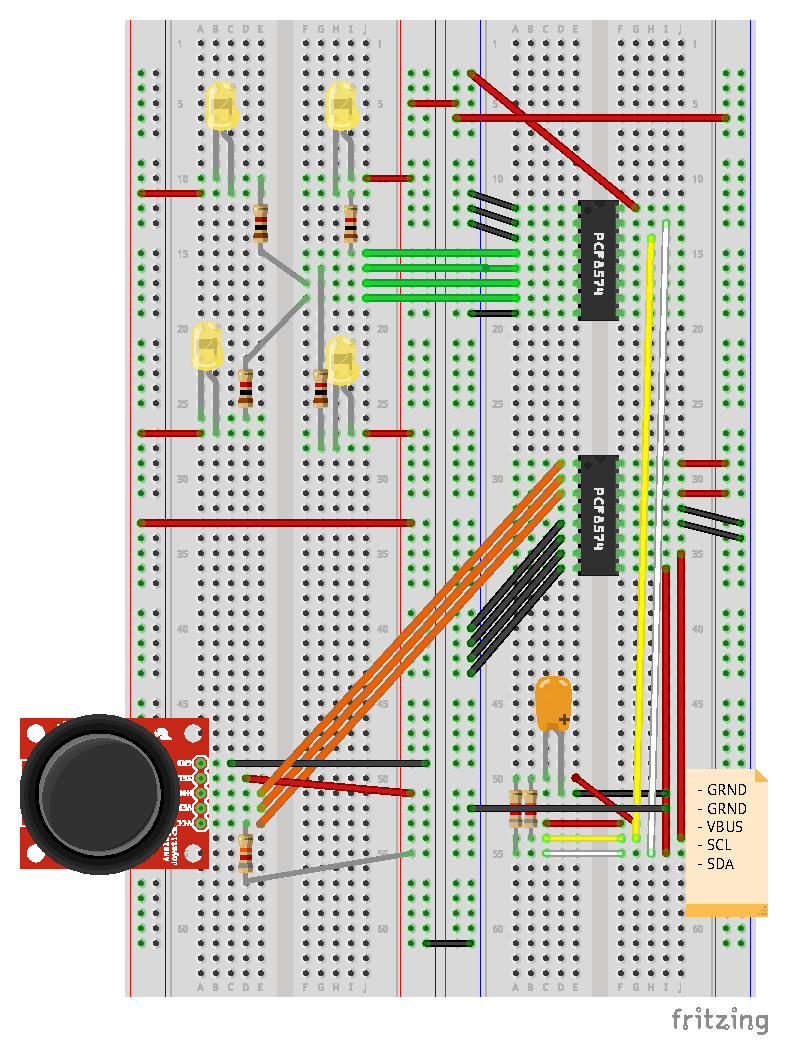
\includegraphics[page=1,width=0.6\textwidth]{Dokumente/Schaltplan.pdf}
	\caption{Hardwareaufbau auf Steckbrett}
	\label{fig:hardwareaufbau}
\end{figure}
\clearpage
\newpage
In Abbildung \ref{fig:hardwareaufbau} ist die finale Erweiterung dargestellt. Folgende Bauteile wurden hierfür verwendet:
\begin{itemize}
	\item PCF8574 Schnittstellen-IC (DIO)
    \item PCF8591 Schnittstellen-IC (ADC)
	\item 4 LEDs
	\item Joystick
\end{itemize}
Der Roboter kann nun über ein Verbindungskabel an das Steckbrett angebunden werden. Hierfür teilen sich die zwei ICs einen I$^2$C-Bus.\\
Die LEDs sind, wie in Abbildung \ref{fig:hardwareaufbau} gezeigt, an den oberen IC angeschlossen. Es werden vier der sieben Digital-IO Pins verwendet.\\
Der Joystick ist, wie in Abbildung \ref{fig:hardwareaufbau} gezeigt, an den unteren IC angeschlossen. Dabei werden zwei Analog-Channels für die beiden Achsen und einer für den Taster verwendet. Der Taster schließt auf GND und braucht deshalb einen Pullup Widerstand (5k, 5V).